\section{Introduction}

Vision-Language-Action (VLA) models \cite{li2024cogact,kim2024openvla,qu2025spatialvla,kim2025fine,zhu2024surveymodelcompressionlarge,zhong2025surveyvisionlanguageactionmodelsaction,black2024pi0visionlanguageactionflowmodel,intelligence2025pi05visionlanguageactionmodelopenworld} have recently emerged as a powerful paradigm for generalist robotic control. Trained on large-scale heterogeneous datasets such as Open-X-Embodiment \cite{vuong2023open}, which aggregate expert demonstrations across diverse robotic tasks, state-of-the-art VLA models exhibit impressive task performance. However, they are typically built on top of large vision–language models \cite{liu2023visual,karamcheti2024prismatic,beyer2024paligemma,steiner2024paligemma}, whose large parameter counts and quadratic-complexity contextual processing \cite{vaswani2017attention} translate into two central deployment bottlenecks: (1) a constrained context budget that limits how many past observations can be ingested, and (2) high per-step inference latency that hinders real-time control. These manifest as the two challenges of \emph{multi-frame integration} and \emph{efficient inference} elaborated below and illustrated in Figure~\ref{fig:intro}.

\noindent\textbf{Multi-frame Integration}. Most current VLAs operate in a memoryless manner \cite{kim2024openvla,li2024cogact,qu2025spatialvla}, taking only the current observation as input. As a result, they struggle with tasks that require temporal dependency or memory tracking. For instance, when instructed to press a button, a VLA must remember whether the button has already been pressed; otherwise, it may repeat the same action indefinitely. A straightforward solution is to include previous observations in the model input. However, VLA's vision backbones typically produce hundreds of visual tokens per image, leading to prohibitively long contexts when multiple frames are concatenated for the transformer-based architecture with quadratic complexity in sequence length. Existing methods often rely on indirect or compressed representations \cite{jang2025contextvla,torne2026mem}, or expose multiple frames to the decoder head only \cite{shi2025memoryvlaperceptualcognitivememoryvisionlanguageaction}, which either risks significant information loss or bypasses the language model’s ability to jointly reason over multiple frames.

\noindent\textbf{Efficient Inference}. Due to their large model sizes, VLAs incur long latency for each forward pass. In real-world settings, however, robotic systems are often expected to respond promptly—for example, a household assistant should complete tasks as quickly as possible, while safety-critical scenarios such as spill containment or fire response may require near-instantaneous reactions. Moreover, recent post-training approaches for VLAs \cite{li2025simplevlarl,lu2025vla}, rely on reinforcement learning \cite{sutton1999policy,schulman2017proximal,shao2024deepseekmath} and require extensive rollouts during training, making inference speed a key bottleneck. While existing work has explored improving VLA efficiency through generic techniques for general machine learning models, such as quantization, token pruning, or layer pruning \cite{xu2025vla,yue2024deer,yang2025efficientvla,kim2024openvla}, these approaches do not leverage the intrinsic characteristics of VLA tasks. Recent works \cite{xu2025vla,liu2025ttf,tan2025think} exploit temporal redundancy by reusing computations across consecutive frames, via KV-cache reuse or action reuse. Nonetheless, these techniques rely on heuristic, non-learnable criteria and often assume that visual similarity in pixel space indicates the temporal-consistency of their latent representations—an assumption that is invalid in transformer-based vision and language backbones, as illustrated in Figure~\ref{fig:related_work1}.

\begin{figure}[t]
    \centering
    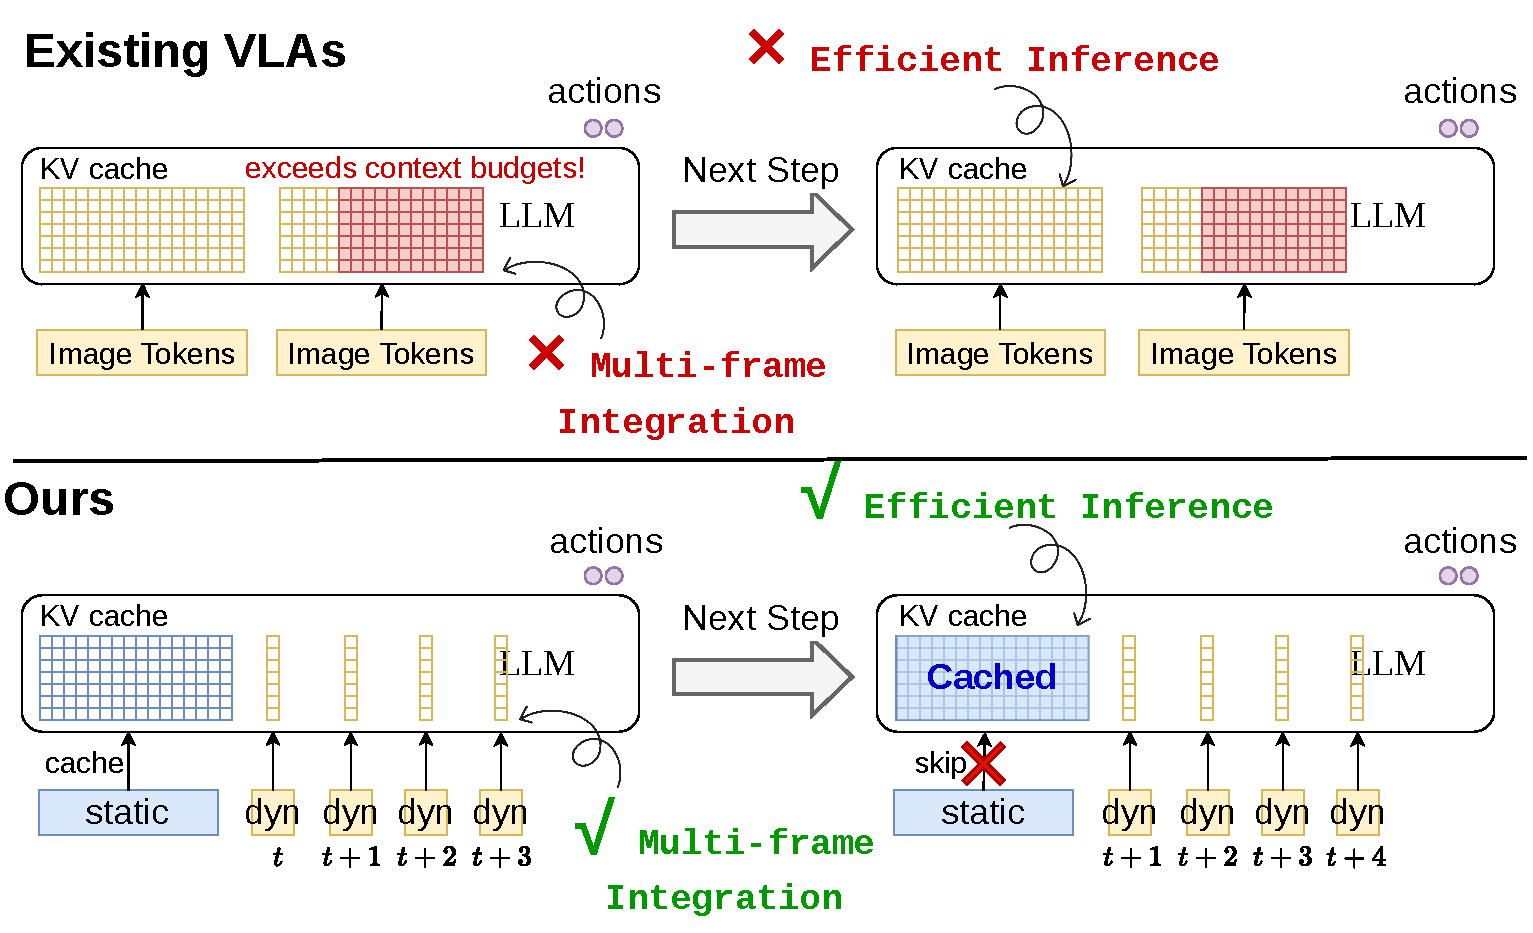
\includegraphics[width=\linewidth]{figs/teaser.pdf}
% \begin{subfigure}[b]{0.4\textwidth}
%     \centering
%     \includegraphics[height=7cm]{figs/teaser1.pdf}
%     \label{fig:0-input}
% \end{subfigure}
% \begin{subfigure}[b]{0.4\textwidth}
%     \centering
%     \includegraphics[height=7cm]{figs/teaser2.pdf}
%     \label{fig:0-input}
% \end{subfigure}
%     \caption{
%         Caption
%     }
\caption{Our model solves two main challenges in existing VLAs with the proposed static-dynamic disentanglement. 1) By keeping one copy of static tokens across all timesteps, our model is able to squash observations of multiple steps to the model's context; 2) By moving static tokens in front of all dynamic tokens, our model could reuse the KV-cache of previous timesteps during rollouts. }
    \label{fig:intro}
\end{figure}

To address these challenges, we propose \dysta{}. We focus on a broad and practically important class of robotic scenarios—such as tabletop manipulation, household chores, and warehouse picking—where the agent operates within relatively stable scenes or undergoes discrete, infrequent scene transitions. In this regime, much of the visual information in a scene remains static or changes slowly over time: the background, objects remaining still, and even moved objects whose visual appearances stay largely invariant. Building on this observation, we explicitly disentangle visual tokens into dynamic tokens and multi-level static tokens with different temporal persistence. This design yields two key benefits. First, instead of conditioning on a single image as in prior work, our model can ingest multi-step observations while maintaining a compact context: static tokens are included only once in the input sequence across timesteps, while only dynamic tokens from multiple steps are concatenated over time. This substantially reduces the effective context length and enables multi-frame integration. Second, our method improves the inference efficiency by reusing key–value (KV) caches associated with static tokens from previous steps. We also introduce a recache gate module that determines whether previously cached static tokens should be reused or recomputed, which further improves performance while minimizing the inference latency.

In addition, we observe that existing simulation benchmarks largely fail to assess a VLA's multi-frame integration capabilities. For example, temporally dependent tasks such as placing objects into a basket do not require remembering past trajectories. To address this gap, we design a new simulation benchmark inspired by principles of human episodic memory, which provides a more effective evaluation of temporal reasoning and memory usage than prior benchmarks \cite{liu2023libero,li2024evaluating}.

To evaluate multi-frame integration, we assess our model on the proposed benchmark. Our method achieves a $24.5\%$ improvement across all metrics and $23.3\%$ in absolute success rate on real-world experiments. To evaluate inference efficiency, we benchmark our approach on public simulation benchmarks~\cite{liu2023libero,li2024evaluating} and real-world experiments. On SimplerEnv~\cite{li2024evaluating}, \dysta{} improves the success rate by $3.9\%$ over the strongest baseline while achieving a $2.26\times$ inference speedup. In real-world experiments, \dysta{} improves the average success rate by $10.6\%$ over the base model and achieves a $2.21\times$ speedup. These results demonstrate that \dysta{} not only enhances multi-frame integration, but also substantially reduces inference latency. In summary, our contributions are as follows:

\begin{itemize}[noitemsep,topsep=0pt,leftmargin=*]
    \item We propose \dysta{}, which enables multi-frame integration and efficient inference by disentangling image tokens to dynamic tokens and multi-level static tokens with different temporal persistence.
    \item We introduce a trainable recache gate that adaptively determines when to refresh the cache or reuse previously cached representations, further improving the performance while minimizing the inference latency.
    \item We introduce LIBERO-Memory, a new benchmark that more effectively evaluates a VLA’s multi-frame integration ability by temporally dependent tasks.
\end{itemize}